\chapter[ಅಧ್ಯಾಯ 6]{}\label{chap6}

\begin{center}
\rule{5cm}{1pt}\\[5pt]
{\Large\bfseries ಸಮಸ್ಯೆಗಳು}\\[3pt]
\rule{5cm}{1pt}
\end{center}

\begin{enumerate}
\renewcommand{\labelenumi}{\bf\theenumi.}
\itemsep=5pt

\item 1 ರಿಂದ 9 ರವರೆಗಿನ ಅಂಕಿಗಳನ್ನು ಒಮ್ಮೆ ಮಾತ್ರ ಬಳಸಿ 99999 ಬರಿಸಿ. ಯಾವುದೇ ಗಣಿತ ಪ್ರಕ್ರಿಯೆ ಬಳಸಬಹುದು. 

\item ಐದು 2 ಬಳಸಿ 7 ಬರಿಸಿ 

\item $1, 3, 5, 7, \cdots$ ಬೆಸ ಸಂಖ್ಯೆಗಳು. ಯಾವುದೇ ಬೆಸ ಸಂಖ್ಯೆಯನ್ನು 3 ಬಾರಿ ಬಳಸಿ, ಸಮ ಸಂಖ್ಯೆ ಬರಿಸಿ. ಯಾವುದೇ ಗಣಿತ ಪ್ರಕ್ರಿಯೆ ಬಳಸಬಹುದು. 

\item 0 ಬಳಸದೆ ಯಾವುದೇ ಎರಡು ಅಂಕಿಗಳನ್ನು 2 ಬಾರಿ ಬಳಸಿ 100 ಬರಿಸಿ. ಯಾವುದೇ ಗಣಿತ ಪ್ರಕ್ರಿಯೆ ಬಳಸಬಹುದು. 

\item ಒಂದೇ ಅಂಕಿಯನ್ನು 3 ಬಾರಿ ಬಳಸಿ 30 ಬರಿಸಿ. ಯಾವುದೇ ಗಣಿತ ಪ್ರಕ್ರಿಯೆ ಬಳಸಬಹುದು. 

\item III ರೇಖೆಗಳನ್ನು ಪುನರ್ಜೋಡಿಸಿ ರಚಿಸ ಬಹುದಾದ ಅತಿ ದೊಡ್ಡ ಸಂಖ್ಯೆ ಯಾವುದು? 

\item IIII ಇವನ್ನು ಪುನರ್ಜೋಡಿಸಿ I ಬರಿಸಿ 

\item ನೂರರ ಮೇಲೆ ಒಂದಕ್ಕೆ ಅರ್ಧ ಡಜನ್ ಕೂಡಿಸಿ, ಮತ್ತೆ 50 ರಿಂದ ಹೆಚ್ಚಿಸಿ ಬರೆದರೆ ಸನ್ನಡತೆಯ ಸೂಚಕ ಲಭ್ಯ. ಹೇಗೆ. 

\item  24 ಬೆಂಕಿಕಡ್ಡಿಗಳಿಂದ ಈ ಕೆಳಗಿನ ಆಕೃತಿಗಳನ್ನು ರಚಿಸಿ. 
\begin{itemize}
\item [(a)] 6 ಕಡ್ಡಿ ಬಾಹು 1 ಚೌಕ
\item [(b)] 3 ಕಡ್ಡಿ ಬಾಹು 3 ಚೌಕಗಳು  
\item [(c)]2 ಕಡ್ಡಿ ಬಾಹು 7 ಚೌಕಗಳು (ಮೂರು 2 ಕಡ್ಡಿ , 4 ಒಂದು ಕಡ್ಡಿ)
\item [(d)]1 ಕಡ್ಡಿ ಬಾಹು 6 ಚೌಕಗಳು  
\item [(e)]1 ಕಡ್ಡಿ ಬಾಹು 7 ಚೌಕಗಳು  
\item [(f)]1 ಕಡ್ಡಿ ಬಾಹು 8 ಚೌಕಗಳು 
\item [(g)]1 ಕಡ್ಡಿ ಬಾಹು 9 ಚೌಕಗಳು 
\end{itemize}

\item ಈ ಗುಣಾಕಾರ ಗಮನಿಸಿ. ಮುಂದಿನ 5 ಹಂತ ಬರೆಯಿರಿ. 

{\fontsize{11pt}{13pt}\selectfont
\begin{tabular}[t]{rcl}
$1 \times 9 + 2$ & = & $11$\\
$12 \times 9 + 3$ & = & $111$\\
$123\times 9 + 4$ & = & $1111$
\end{tabular}}\relax

\item ಎಡದಿಂದ ಬಲಕ್ಕೆ ಅಥವಾ ಬಲದಿಂದ ಎಡಕ್ಕೆ ಓದಿದಾಗಲೂ ಸಂಖ್ಯೆ ಬದಲಾಗದಿದ್ದರೆ ಅದನ್ನು ಮಾಲಾ ಸಂಖ್ಯೆ (Palindrome number) ಎನ್ನುತ್ತಾರೆ. ಉದಾ: 2112 ಕ್ರಿ.ಶ. 9ನೆ ಶತಮಾನದಲ್ಲಿದ್ದ ಮಹಾವೀರಾಚಾರ್ಯರು ತಮ್ಮ ಕೃತಿ ``ಗಣಿತ ಸಾರ\break ಸಂಗ್ರಹ"ದಲ್ಲಿ ಕೆಲವು ಮಾಲಾ ಸಂಖ್ಯೆ ಉದಾಹರಿಸಿದ್ದಾರೆ. 

\begin{tabular}[t]{ccl}
$134\times 109$ & = & $15151$\\
$142857143\times 7$ & = & $1000000001$\\
$333333666667\times 33$ & = & $11000011000011$
\end{tabular}

ಬರೆಯುವ ಸಾಮಗ್ರಿಗಳಾದ ಕಾಗದ, ಲೇಖನಿ ಇಲ್ಲದಿದ್ದ ಕಾಲದಲ್ಲಿ ಇವುಗಳ ರಚನೆ ಏಕೆ, ಹೇಗೆ ಎಂಬುದು ಕುತೂಹಲಕಾರಿ 

\item ಈ ಗುಣಾಕಾರ ಗಮನಿಸಿ. ಮುಂದಿನ 5 ಹಂತ ಬರೆಯಿರಿ. 

\begin{tabular}[t]{rcl}
$8\times 8 + 13$ & = & $77$\\
$88\times 8 + 13$ & = & $717$\\
$888\times 8 + 13$ & = & $7117$\\
$8888\times 8 + 13$ & = & $71117$
\end{tabular}

\item ಈ ಸಂಖ್ಯಾ ವಿಚಿತ್ರ ನೋಡಿ. 15873ನ್ನು 7ರ ಮಗ್ಗಿ ಸಂಖ್ಯೆಗಳಿಂದ ಗುಣಿಸಿ, ಲಬ್ಧವನ್ನು 3ರ ಮಗ್ಗಿ ಸಂಖ್ಯೆಗಳಿಂದ ಭಾಗಿಸಿ. 

\begin{tabular}[t]{ccccc}
\qquad 7ರ ಮಗ್ಗಿ &  & \qquad 3ರ ಮಗ್ಗಿ & & \\
$15873\times 7$ & = & $111~111\div 3$ & = & $37037$\\
$15873\times 14$ & = & $222~222\div 6$ & = & $37037$\\
$15873\times 21$ & = & $333~333\div 9$ & = & $37037$
\end{tabular}

ಮುಂದಿನ ಹಂತಗಳನ್ನು ಬರೆಯಿರಿ. 

\item ಈ ಆಕೃತಿಯನ್ನು 3 ಸರಳರೇಖೆಗಳಿಂದ ಕತ್ತರಿಸಿ 9 ತ್ರಿಭುಜ ಬರಿಸಿ. 
\begin{figure}[H]
\centering
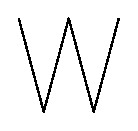
\includegraphics{images/chap6/q14.eps}
\end{figure}

\item ಈ ಆಕೃತಿಯಲ್ಲಿರುವ ಆಯತಗಳೆಷ್ಟು? 
\begin{figure}[H]
\centering
\includegraphics{images/chap6/q15.eps}
\end{figure}

\item ಪೆನ್ಸಿಲ್ ಎತ್ತದೆ, ಕಾಗದ ಮಡಿಸದೆ, ಯಾವುದೇ ರೇಖೆಯ ಮೇಲೆ 2 ಬಾರಿ ಚಲಿಸದೆ, ಹಿಮ್ಮುಖವಾಗಿ ಹೋಗದೆ, ಈ ಚಿತ್ರದ ಎಲ್ಲ ಬಾಹುಗಳ ಮೇಲೆ ಚಲಿಸಿ. 
\begin{figure}[H]
\centering
\includegraphics{images/chap6/q16.eps}
\end{figure}

\item ಬಾಲೇ ಮರಾಲ ಕುಲ ಮೂಲದಲಾನಿ ಸಪ್ತ 

ತೀರೇ ವಿಲಾಸಭರ ಮಂಥರ ಗಾಣ್ಯ ಪಶ್ಯಂ 

ಕುರ್ವಂಚ ಕೇಲಿ ಕಲಹಂ ಕಲಹಂಸಯುಗ್ಮಂ 

ಶೇಷಂ ಜಲೇ ವದ ಮರಾಲ ಕುಲ ಪ್ರಮಾಣಂ ।

\smallskip
\hfill (ಭಾಸ್ಕರಾಚಾರ್ಯರ `ಲೀಲಾವತೀ'ಯಿಂದ)

\smallskip
{\bf ಅರ್ಥ:} ಎಲೆಬಾಲೆ, ಜಲವಿಲಾಸ ಸಾಕಾಗಿ ಒಂದು ಹಂಸ ಸಮೂಹದಲ್ಲಿ ವರ್ಗ ಮೂಲದ ಮೂರೂವರೆಯಷ್ಟು ಹಂಸಗಳು ದಡಕ್ಕೆ ಹೋದುವು. ಒಂದು ಜೋಡಿ ಮಾತ್ರ ಇನ್ನೂ ಕೇಲಿ ಕಲಹ ಮಾಡುತ್ತ ನೀರಿನಲ್ಲೇ ಇದ್ದು, ದಡಕ್ಕೆ ಹೋದ ಹಂಸಗಳನ್ನು ನೋಡುತ್ತ ಇದ್ದುವು. ಸಮೂಹದಲ್ಲಿದ್ದ ಹಂಸಗಳ ಸಂಖ್ಯೆ ಎಷ್ಟು? 

\item ಚರತಿ ಕಮಲ ಷಂಡೇ ಸಾರಸಾನಾಂ ಚತುರ್ಥೋ 

ನವಮ ಚರಣ ಭಾಗೌ ಸಪ್ತ ಮೂಲಾನಿ ಚಾದ್ರೌ 

ವಿಕಚ ವಕುಲ ಮಧ್ಯೇ ಸಪ್ತ ನಿಘ್ನಾಷ್ಟ ಮಾನಾಃ 

ಕತಿ ಕಥಯ ಸಂಖ್ಯೇ ತ್ವಂ ಪಕ್ಷಿಣೋ ದಕ್ಷ ಸಾಕ್ಷಾತ್ 

\smallskip
\hfill (ಭಾಸ್ಕರಾಚಾರ್ಯರ `ಲೀಲಾವತೀ'ಯಿಂದ)

\smallskip
{\bf ಅರ್ಥ:} ಸಾರಸ ಪಕ್ಷಿಗಳ $\dfrac{1}{4}$ ಭಾಗವು ಕಮಲ ಪುಷ್ಪಗಳ ಮಧ್ಯದಲ್ಲಿ ಚಲಿಸುತ್ತಿವೆ. $\dfrac{1}{9}$ ಭಾಗ, $\dfrac{1}{4}$ ಭಾಗ ಮತ್ತು ವರ್ಗ ಮೂಲದ ಏಳರಷ್ಟು ಬೆಟ್ಟದ ಮೇಲೆ ಇದೆ. ಉಳಿದ 56 ಪಕ್ಷಿಗಳು ನಕುಲ ವೃಕ್ಷಗಳ ನಡುವೆ ಇದೆ. ಪಕ್ಷಿಗಳ ಒಟ್ಟು ಸಂಖ್ಯೆ ಎಷ್ಟು? 

\smallskip
\item ಒಬ್ಬ ರೈತನಿಗೆ ಚೌಕಾಕಾರದ ತೋಟವಿದೆ. ಸುತ್ತಲೂ ತಂತಿ ಬೇಲಿ ಹಾಕಿಸಲು ಕಂಭ ನೆಡಿಸಿದ. ಪ್ರತಿ ಪಕ್ಕದಲ್ಲಿಯೂ 12 ಕಂಭಗಳು ಸಮಾನ ದೂರದಲ್ಲಿರುವಂತೆ ನೆಡಿಸಿದ. ಒಟ್ಟು ಕಂಭಗಳೆಷ್ಟು?

\item ಒಂದು ಗಡಿಯಾರ 4 ಗಂಟೆ ಹೊಡೆಯಲು 6 ಸೆ. ತೆಗೆದುಕೊಳ್ಳುತ್ತದೆ. 12 ಗಂಟೆ ಹೊಡೆಯಲು ಎಷ್ಟು ಸಮಯ ಬೇಕು? 

\item ನಾಲ್ಕಂಕಿಯ 2 ಸಂಖ್ಯೆ ಬರೆಯಲು ಹೇಳಿ. ಅದರ ಕೆಳಗೆ ನೀವೂ ನಾಲ್ಕಂಕಿಯ 2\break ಸಂಖ್ಯೆ  ಬರೆಯಿರಿ. ಉತ್ತರ ದಿಢೀರ್ ಹೇಳಿ

\item ಒಂದು ಸ್ತಂಭಾಕೃತಿ ಬಾಟಲಿನಲ್ಲಿ ಸುಮಾರು ಅರ್ಧಭಾಗದಷ್ಟು ನೀರಿದೆ. ಅ ಬಾಟಲಿನ ತಳ ಮಟ್ಟಸವಾಗಿದೆ. ಒಂದು ಅಳತೆ ಪಟ್ಟ ಕೊಟ್ಟಿದೆ. ಬಾಟಲಿಗೆ ಹಾಕಿರುವ ಮುಚ್ಚಳ ತೆಗೆಯದೆ, ಬಾಟಲಿನ ಹಿಡಿಪು (capacity) - ಒಳಗಾತ್ರ ಲೆಕ್ಕಿಸಿ. 

\item 10 ಸೇಬುಗಳನ್ನು 5 ಸರಳ ರೇಖೆಗಳ ಮೇಲೆ ಜೋಡಿಸಿ. ಪ್ರತಿ ರೇಖೆಯ ಮೇಲೂ 4 ಸೇಬು ಬರಬೇಕು. 

\item ವೃತ್ತಾಕಾರದ ರೊಟ್ಟಿ ಇದೆ. 4 ಸರಳ ರೇಖೆ ಎಳೆದು ಕತ್ತರಿಸಿ. 11 ಚೂರು ಬರಬೇಕು. ಚೂರುಗಳು ಸಮವಾಗಿರಬೇಕಾಗಿಲ್ಲ. 

\item 175 ಸೆಂ.ಮೀ ಎತ್ತರದ ವ್ಯಕ್ತಿಯೊಬ್ಬನು ಭೂಮಿಯ ಸುತ್ತ ಸಮಭಾಜಕ ವೃತ್ತದ ಮೇಲೆ ನಡೆಯುತ್ತಾನೆ. ಅವನ ಪಾದಗಳಿಗಿಂತ ತಲೆ ದೊಡ್ಡ ವೃತ್ತ ರಚಿಸಿರುತ್ತದೆ. ಅವನು 1 ಸುತ್ತು ಸುತ್ತಿದಾಗ ಪಾದ ವೃತ್ತಕ್ಕೂ ತಲೆ ವೃತ್ತಕ್ಕೂ ಇರುವ ಉದ್ದದ ವ್ಯತ್ಯಾಸವೆಷ್ಟು? 

\eject

\item ಒಬ್ಬ ವ್ಯಾಪಾರಿ ಒಂದು ದಿನ ತನ್ನ ಅಂದಿನ ಗಳಿಕೆ ಹಣ ಎಣಿಸುತ್ತಿದ್ದ, ಅದರಲ್ಲಿ 100 ಒಂದು ರೂಪಾಯಿ ನಾಣ್ಯ ಇತ್ತು. ಎಣಿಸುವಾಗ ಹತ್ತು ನಾಣ್ಯಗಳು ಉಳಿದವುಗಳಿಗಿಂತ ಭಿನ್ನವಾಗಿದ್ದುದು ಕಂಡು ಬಂದಿತು. ಸೂಕ್ಷ್ಮವಾಗಿ ಗಮನಿಸಿದಾಗ ಆ ಹತ್ತು ಖೋಟಾ ಆಗಿರುವುದು ತಿಳಿಯಿತು. ಎಲ್ಲ ನಾಣ್ಯಗಳನ್ನು 10ರ ರಾಶಿ (Pile)ಗಳಾಗಿ ಇರಿಸಿದ. ಒಂದು ಪೂರ್ತಿರಾಶಿ ಖೋಟಾ ಆಗಿತ್ತು. ಖೋಟಾ ನಾಣ್ಯ 11ಗ್ರಾಂ ಸಾಚಾ ನಾಣ್ಯ 10ಗ್ರಾಂ ಇದೆ ಎಂದೂ ಪತ್ತೆಮಾಡಿದ. ಆ ವೇಳೆಗೆ ಅವನ ಗೆಳಯ$-$ಗಣಿತಾಸಕ್ತ ಅಲ್ಲಿಗೆ ಬಂದ. ವ್ಯಾಪಾರಿಯು ವಿನೋದಕ್ಕಾಗಿ ಹೇಳಿದ. ತ್ರಾಸು, ಬಟ್ಟು ಬಳಸಿ ಒಂದೇ ತೂಕದಲ್ಲಿ ಖೋಟಾ ನಾಣ್ಯದ ರಾಶಿ ಪತ್ತೆ ಮಾಡಿದರೆ, ಎಲ್ಲವೂ ನಿನಗೆ. ಗೆಳೆಯ ಗೆದ್ದ ಹೇಗೆ?

\item ಕೆಲವು ಸಂಖ್ಯೆಗಳ ಅಪವರ್ತನಗಳ ಮೊತ್ತ ವರ್ಗ ಸಂಖ್ಯೆಯಾಗಿರುತ್ತದೆ. ಇಂತಹವನ್ನು ಪತ್ತೆ ಮಾಡುವುದೇ ಮೋಜು 

ಉದಾ:

\begin{tabular}[t]{llll}
& ಸಂಖ್ಯೆ  \quad ಅಪವರ್ತನಗಳು & ಮೊತ್ತ & \\
 & $3$ \quad\qquad $3, 1$ & $3 + 1 = 4$ & $2^{2}$\\
$66$ & $1+2+3+6+11+22+33+66$ & $144$ & $12^{2}$
\end{tabular}

\vskip 0.3cm
ಇದೇರೀತಿ ಸಂಖ್ಯೆಗಳು $70, 81, 1501, 400 \cdots$ ಇವುಗಳನ್ನು ಪರಿಶೀಲಿಸಿ. ಬೇರೆ ಸಂಖ್ಯೆ ಆವಿಷ್ಕರಿಸಲು ಪ್ರಯತ್ನಿಸಿ. 

\item ಕಾಪರೇಕರ್ ಸ್ಥಿರಾಂಕ 6174

ಯಾವುದೇ ನಾಲ್ಕಂಕಿಯ ಸಂಖ್ಯೆ ತೆಗೆದುಕೊಳ್ಳಿ. ಅಂಕಿಗಳು ಕನಿಷ್ಥ ಒಂದಾದರೂ ಬೇರೆಯದಿರಬೇಕು. ಇದನ್ನು ಇಳಿಕೆ ಕ್ರಮದಲ್ಲಿ ಬರೆಯಿರಿ. ತಿರುವು ಮುರುವು ಮಾಡಿ, ಬಂದ ಸಂಖ್ಯೆಯನ್ನು ಮೊದಲಿನದರಲ್ಲಿ ಕಳೆಯಿರಿ. ಇದೇ ಪ್ರಕ್ರಿಯೆ ಮುಂದುವರಿಸಿ. ಅಂತಿಮ ಉತ್ತರ ಯಾವಾಗಲೂ 6174

ಉದಾ: (1)
\begin{equation*}
\begin{tabular}[t]{r}
1000 \\
0001\\\cline{1-1} 
0999
\end{tabular}
\quad
\begin{tabular}[t]{r}
9990\\ 
0999\\\cline{1-1} 
8991
\end{tabular}
\quad
\begin{tabular}[t]{r}
9981\\ 
1899\\\cline{1-1} 
8082
\end{tabular}
\quad
\begin{tabular}[t]{r}
8820\\ 
0288\\\cline{1-1} 
8532
\end{tabular}
\quad
\begin{tabular}[t]{r}
8532\\ 
2358\\\cline{1-1} 
9174
\end{tabular}
\quad
\begin{tabular}[t]{r}
7641\\ 
1467\\\cline{1-1} 
6174
\end{tabular}
\end{equation*}

ಉದಾ: (2) 5427
\begin{equation*}
\begin{tabular}[t]{r}
7542 \\
2457\\\cline{1-1} 
5085
\end{tabular}
\quad
\begin{tabular}[t]{r}
8550\\ 
0558\\\cline{1-1} 
8992
\end{tabular}
\quad
\begin{tabular}[t]{r}
9982\\ 
2899\\\cline{1-1} 
7083
\end{tabular}
\quad
\begin{tabular}[t]{r}
8730\\ 
0378\\\cline{1-1} 
8352
\end{tabular}
\quad
\begin{tabular}[t]{r}
8532\\ 
2358\\\cline{1-1} 
6174
\end{tabular}
\end{equation*}

\{ಕಳೆದ ಶತಮಾನದಲ್ಲಿ ಮಹಾರಾಷ್ಟ್ರದಲ್ಲಿ ಗಣಿತ ಶಿಕ್ಷಕರಾಗಿದ್ದ ಡಿ. ಆರ್. ಕಾಪರೇಕರ್‌ರವರು ಆವಿಷ್ಕರಿಸಿದುದು\}

\item  ಒಂದು ವರ್ಗ ಸಂಖ್ಯೆಯನ್ನು 11 ರಿಂದ ಗುಣಿಸಿ, 1ನ್ನು ಕೂಡಿಸಿದರೆ ಇನ್ನೊಂದು ವರ್ಗ ಸಂಖ್ಯೆ ಲಭ್ಯ. ಮೊದಲ ವರ್ಗ ಸಂಖ್ಯೆ ಯಾವುದು? 

\item ಪ್ರತಿ ಚಿಹ್ನೆಯು ಒಂದು ಸಂಖ್ಯೆಯನ್ನು ಸೂಚಿಸುತದೆ. ಅಡ್ಡ ಸಾಲಿನ, ಕಂಭ ಸಾಲಿನ ಸಂಖ್ಯೆಗಳ ಮೊತ್ತ ಬರೆದಿದೆ. 
\begin{figure}[H]
\centering
\includegraphics{images/chap6/q30.eps}
\end{figure}

? ಇರುವಲ್ಲಿರಬೇಕಾದ ಸಂಖ್ಯೆಯನ್ನು ಲೆಕ್ಕಿಸಿ. 
\end{enumerate}

\smallskip

\begin{center}
\rule{5cm}{1pt}\\[3pt]
{\Large\bfseries ಉತ್ತರಗಳು}\\[-0.1cm]
\rule{5cm}{1pt}
\end{center}

\begin{enumerate}
\itemsep=5pt

\item $98765 + 1234 = 99999$

\item 
\begin{tabular}{@{}l@{$\;$}c@{\hspace{1.5cm}}l@{$\;$}c}
(a) & $2 + \dfrac{2}{2} + 2^{2} = 7$ & 
(b) & $2 +2 + 2 + \dfrac{2}{2} = 7$ 
\end{tabular}


\item $1 + \dfrac{1}{1} = 2; \quad 3 + \dfrac{3}{3} = 4;\quad 5 + \dfrac{5}{5} = 6$

\item $99 + \dfrac{2}{2} = 100;\quad 99 + \dfrac{3}{3} = 100$ ಇತ್ಯಾದಿ. 

\item $33 - 3 = 30; ~~ 3^{3} + 3 = 30; ~~ 5 \times 5 + 5 = 30;  ~~ 6 \times 6 - 6 = 30$;\break  ~$X + X + X = 30$

\item
~

\begin{tabular}[t]{cc}
\includegraphics[scale =1.1]{images/chap6/ans6.eps} & \raisebox{.1cm}{= $50,000$ \{$L = 50$ ಮೇಲುಗೆರೆ ಎಳೆದರೆ $10,000$ ಪಟ್ಟು\}}
\end{tabular}

\item
~

\begin{tabular}[t]{cc}
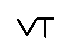
\includegraphics[scale=1.1]{images/chap6/ans7.eps} & \raisebox{.1cm}{$= 1$}
\end{tabular}

\item ನೂರರ ಮೇಲೆ ಒಂದು ನೂರು $C +$ ಒಂದು $C I$

ಅರ್ಧಡಜನ್ $\dfrac{12}{2} = 6 = VI\qquad CIVI$

$50$ನ್ನು ಕೂಡಿಸಿ $50 = L\qquad CIVIL$

\item
\begin{itemize}
\item[(a)] 
~

\begin{figure}[H]
\centering
\includegraphics{images/chap6/ans9a.eps}
\end{figure}

\item[(b)] 2 ವಿಧಾನಗಳಿವೆ 
~

\begin{figure}[H]
\centering
\includegraphics{images/chap6/ans9b.eps}
\end{figure}

\item[(c)]
~

\begin{minipage}[c]{5cm}
\begin{figure}[H]
\centering
\includegraphics[scale=0.9]{images/chap6/ans9c.eps}
\end{figure}
\end{minipage}
\begin{minipage}[c]{4cm}
{\fontsize{11pt}{13pt}\selectfont
\begin{equation*}
\left.
\begin{aligned}
\text{ABCD}\\
\text{EFGH}\\
\text{IJKL}
\end{aligned}
\right\}
~~  \text{2 ಕಡ್ಡಿ ಚೌಕಗಳು}
\end{equation*}}\relax
\end{minipage}

EFGH ಒಳಗಿರುವುದು 4 ಒಂದು ಕಡ್ಡಿ 

\item[(d)]
~

\begin{figure}[H]
\centering
\includegraphics{images/chap6/ans9d.eps}
\end{figure}

\item[(e)]
~

\begin{figure}[H]
\centering
\includegraphics{images/chap6/ans9e.eps}
\end{figure}

\item[(f)] ಎರಡು ವಿಧಾನಗಳಿವೆ 
\begin{figure}[H]
\centering
\includegraphics{images/chap6/ans9f.eps}
\end{figure}

\item[(g)]
~

\begin{figure}[H]
\centering
\includegraphics{images/chap6/ans9g.eps}
\end{figure}
\end{itemize}

\item
\begin{tabular}[t]{rcl}
$1234\times 9 + 5$ & = & $11111$\\
$12345\times 9 + 6$ & = & $111111$\\
$123456\times 9 + 7$ & = & $1111111$\\
$1234567\times 9 + 8$ & = & $11111111$\\
$12345678\times 9 + 9$ & = & $111111111$
\end{tabular}

\item ಉತ್ತರದ ಅಗತ್ಯವಿಲ್ಲ

\item
{\fontsize{11pt}{13pt}\selectfont
\begin{tabular}[t]{rcl}
$88888\times 8 + 13$ & = & $711117$\\
$888888\times 8 + 13$ & = & $7111117$\\
$8888888\times 8 + 13$ & = & $71111117$\\
$88888888\times 8 + 13$ & = & $711111117$\\
$888888888\times 8 + 13$ & = & $7111111117$
\end{tabular}}\relax

\item
{\fontsize{11pt}{13pt}\selectfont
\begin{tabular}[t]{lllll}
$15873\times 28$ & = & $444444\div 12$ & = $37037$\\
$15873\times 35$ & = & $555555\div 15$ & = $37037$\\
$15873\times 42$ & = & $666666\div 18$ & = $37037$\\
$15873\times 49$ & = & $777777\div 21$ & = $37037$\\
$15873\times 56$ & = & $888888\div 24$ & = $37037$\\
$15873\times 63$ & = & $999999\div 27$ & = $37037$
\end{tabular}}\relax

\item
~
\vskip -0.4cm
\begin{figure}[H]
\centering
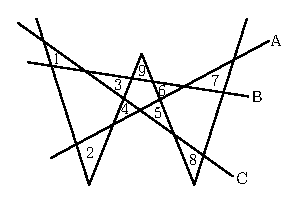
\includegraphics[scale=1.0]{images/chap6/ans14.eps}
\end{figure}

A, B, C, ಸರಳ ರೇಖೆಗಳು 

\item
~

\begin{figure}[H]
\centering
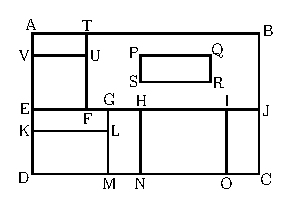
\includegraphics[scale=1.0]{images/chap6/ans15.eps}
\end{figure}

{\fontsize{11pt}{13pt}\selectfont
\begin{tabular}[c]{cccc}
ABCD & ATUV & EHND & GIOM\\
ABJE & VUFE & EIOD & GJCM\\
ATFE & EGLK & EJCD & HION\\
TBJF & KLMD & KLMD & HJCN\\
PQRS & EGMD & GHNM & IJCO\\
\end{tabular}}\relax

\smallskip
ಒಟ್ಟು 20 ಆಯತಗಳು 

\item ಪೆನ್ಸಿಲ್ ಎತ್ತದೆ, ಕಾಗದ ಮಡಿಸದೆ, ಯಾವುದೇ ರೇಖೆಯ ಮೇಲೆ 2 ಬಾರಿ ಚಲಿಸದೆ, ಹಿಮ್ಮುಖವಾಗಿ ಹೋಗದೆ ಈ ಚಿತ್ರದ ಎಲ್ಲ ಬಾಹುಗಳ ಮೇಲೆ ಚಲಿಸಿ. 
\begin{figure}[H]
\centering
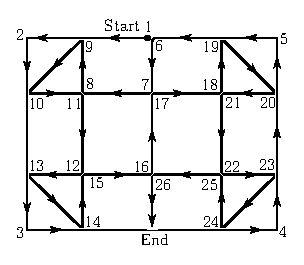
\includegraphics[scale=1.4]{images/chap6/ans16.eps}
\end{figure}

\item ಹಂಸಗಳ ಸಂಖ್ಯೆ $x$ ಇರಲಿ 

\begin{tabular}{l|l}
$3\dfrac{1}{2} \sqrt{x} + 2 = x$ & $\dfrac{7}{2} \sqrt{x} + 2 = x$\\[0.1cm]
ಇದನ್ನು ಬಿಡಿಸಿದಾಗ $x = 16$ & $7\sqrt{x} + 4 = 2x$\\[0.1cm]
& $7\sqrt{x} = 2x - 4$\\[0.1cm]
& $(7\sqrt{x})^{2} = (2x - 4)^{2}$\\[0.1cm]
& $49x = 4x^{2} - 16x + 16$\\[0.1cm]
& $4x^{2} - 65x + 16 = 0$\\[0.1cm]
& $(4x - 1) (x - 16) = 0$\\[0.1cm]
& $x= 16$\quad ಅಥವಾ \quad $\dfrac{1}{4}$\\[0.1cm]
& $\therefore\quad$ ಹಂಸಗಳು 16
\end{tabular}

\smallskip
\item ಸಾರಸ ಪಕ್ಷಿಗಳ ಸಂಖ್ಯೆ $x$ ಇರಲಿ 

$\dfrac{x}{4} + \dfrac{x}{9} + \dfrac{x}{4} + 7\sqrt{x} + 56 = x$

36 ರಿಂದ ಗುಣಿಸಿ $9x + 4x + 9x + 252\sqrt{x} + 2016 = 36x$
\begin{align*}
252\sqrt{x} + 2016 & = 14x\\
18\sqrt{x} + 144 & = x\\
x - 144 & 18\sqrt{x}\\
(x - 144)^{2} & = 324x\\
x^{2} - 612x + 20376 & = 0\\
(x - 576) (x - 36) & = 0\\
x = 576\quad \text{ ಅಥವಾ}\quad 36 & 
\end{align*}

$36$ ಸರಿಯಾಗುವುದಿಲ್ಲ $\quad\therefore~ 56$ ಉಳಿಯುತ್ತದೆ. 

$\therefore~$ ಸಾರಸಗಳ ಸಂಖ್ಯೆ  $576$

\item 44

\item $22$ ಸೆ. $4$ಗಂ ಹೊಡೆಯಲು $3$ ಅವಧಿಗಳು $6$ ಸೆಕೆಂಡ್‌ಗಳು 

$\therefore~ 1$ ಅವಧಿಗೆ $2$ ಸೆ.

12 ಗಂಟೆ ಹೊಡೆಯಲು 11 ಅವಧಿಗಳು 

$\therefore~ 11\times 2 = 22$ ಸೆ. 

\item ಉತ್ತರ ಯಾವಾಗಲೂ 19998

ನೀವು ಬರೆಯುವ 2 ಸಂಖ್ಯೆಗಳು ಅವರು ಬರೆದ ಸಂಖ್ಯೆಗಳ 9ರ ಪೂರಕವಾಗಬೇಕು. 

ಉದಾ: 
\begin{align*}
& \left.
\begin{aligned}
7682 \\
5436
\end{aligned}
\right\}
~~  \text{ಅವರ ಸಂಖ್ಯೆಗಳು}\\
& \left.
\begin{aligned}
2317\\
4563\\
\hline
19998\\
\hline
\end{aligned}
\right\}
~~  \text{ನಿಮ್ಮ ಸಂಖ್ಯೆಗಳು}
\end{align*}

$7 + 2 = 9$,~  $6 + 3 = 9$,~ $8 + 1 = 9$,~ $2 + 7 =9$ ಇತ್ಯಾದಿ 

\item ಕೊಟ್ಟಿರುವ ಬಾಟಲು `ಎ' ಇರಲಿ ಅದರ ನೀರಿನ ಎತ್ತರ ಅಳೆಯಿರಿ. $h_{1}$ ಇರಲಿ. 

ಬಾಟಲಿಯನ್ನು ತಲೆ ಕೆಳಗು ಮಾಡಿ `ಬಿ' ನೋಡಿ 

ನೀರಿನ ಮೇಲ್ಮೈನಿಂದ ಖಾಲಿ ಬಾಟಲ್ ಖಾಲಿ ಜಾಗದ ಎತ್ತರ ಅಳೆಯಿರಿ $h_{2}$ ಇರಲಿ. 

\begin{figure}[H]
\centering
\includegraphics{images/chap6/ans22.eps}
\end{figure}

ಬಾಟಲಿ ಪಾದದ ವೃತ್ತದ ತ್ರಿಜ್ಯ ಅಳೆಯಿರಿ. $r$ ಇರಲಿ (ವ್ಯಾಸ ಅಳೆದು ಅರ್ಧಿಸಿ)

\smallskip
ಬಾಟಲಿಯ ಒಳಗಾತ್ರ = $\Pi r^{2} (h_{1} + h_{2})$

\item ಪ್ರತಿ ಬಾಹುವಿನ ಮೇಲೂ 4 ಸೇಬುಗಳಿವೆ. 

ಒಟ್ಟು 5 ಬಾಹುಗಳಿವೆ. ಹಾಗೂ 10 ಸೇಬುಗಳಿವೆ. 

\begin{figure}[H]
\centering
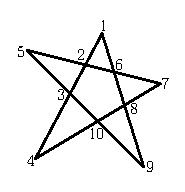
\includegraphics[scale=1.1]{images/chap6/ans23.eps}
\end{figure}


\item
~

\begin{figure}[H]
\centering
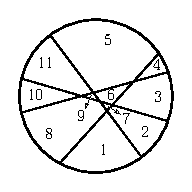
\includegraphics[scale=1.3]{images/chap6/ans24.eps}
\end{figure}

\item ಭೂಮಿಯ ತ್ರಿಜ್ಯ $r$ ಇರಲಿ. 

\vskip 0.1cm
ಪಾದವು ಸುತ್ತುವ ದೂರ $2\Pi r$

\vskip 0.1cm
ತಲೆ ಸುತ್ತುವ ದೂರ $2\Pi (r + 175)$

\vskip 0.1cm
ವ್ಯತ್ಯಾಸ $2\Pi (r + 175) - 2\Pi r$

\vskip 0.1cm
$2\Pi r + 2\Pi\times 175 - 2\Pi r$

\vskip 0.3cm
$= 2\times \dfrac{22}{\cancel{7}} \times \cancel{175}^{25} = 44\times 25 = 1100$ ಸೆ. ಮೀ 

\item ತ್ರಾಸಿನ ತಟ್ಟೆಯಲ್ಲಿ ಒಂದನೆ ರಾಶಿಯಿಂದ 1, ಎರಡನೆ ರಾಶಿಯಿಂದ 2 ಹೀಗೆ 10ನೆ ರಾಶಿ ಪೂರ್ತಿ ನಾಣ್ಯಗಳನ್ನು ಪ್ರತ್ಯೇಕವಾಗಿ ಇರಿಸಿದ. ತೂಕ ಕಂಡು ಹಿಡಿದ. 

\vskip 0.1cm
ತಟ್ಟೆಯಲ್ಲಿದ್ದ ಒಟ್ಟು ನಾಣ್ಯಗಳ ಸಂಖ್ಯೆ $1 +2 + 3 + \cdots + 10 = \frac{11 + 10}{2} = 55$

\vskip 0.1cm
ಎಲ್ಲವೂ ಸಾಚಾ ಆಗಿದ್ದರೆ ತೂಕ $55\times 10 = 550$ಗ್ರಾಂ 

\vskip 0.1cm
ಎಷ್ಟು ಗ್ರಾಂ ಹೆಚ್ಚಿದೆ ಅಷ್ಟನೆಯ ರಾಶಿ ಖೋಟಾ ಎಂದು ನಿರ್ಧರಿಸಿದ 

\item 
{\fontsize{11pt}{13pt}\selectfont
\begin{tabular}[t]{lll}
$70$ & $1+2+5+7+20+24+35+70$  & $= 144 = 12^{2}$\\
$81$  & $1+3+9+27+81$  & $= 121 = 11^{2}$\\
$1501$  & $1 +19+79+1501$  & $= 1600 = 40^{2}$
\end{tabular}}\relax

\vskip 0.1cm

\item ಉತ್ತರದ ಅಗತ್ಯವಿಲ್ಲ 

\item ಮೊದಲ ವರ್ಗ ಸಂಖ್ಯೆ $x^{2}$ ಇದ್ದರೆ $11x^{2} + 1 = y^{2}$ ಲಭಿಸುತ್ತದೆ. 

$x = 3$, $y = 10$ ಆದಾಗ ಸಮೀಕರಣ ಬಿಡಿಸಿದಂತಾಗುತ್ತದೆ. 

$\therefore$~ಮೊದಲ ಸಂಖ್ಯೆ  3

\item  ಸೌಕರ್ಯಕ್ಕಾಗಿ ಚಿತ್ರಗಳಿಗೆ ಅಕ್ಷರ ಕೊಡೋಣ 

\begin{minipage}[c]{4cm}
\begin{figure}[H]
\centering
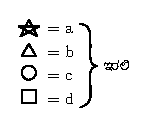
\includegraphics[scale=1.1]{images/chap6/ans30.eps}
\end{figure}
\end{minipage}
\begin{minipage}[c]{4cm}
\begin{figure}[H]
\centering
\includegraphics{images/chap6/q30.eps}
\end{figure}
\end{minipage}

ಈ ಕೆಳಗಿನ ಸಮೀಕರಣಗಳು ಸಿದ್ಧಿಸುತ್ತದೆ. 
\begin{equation*}
\begin{aligned}
a+b+c+c=66\\
a+a+b+b=68\\
d+d+d+a=74\\
a+a+c+d=74\\
c+b+c+d=64\\
c+b+b+a=64
\end{aligned}
\qquad\text{ ಅಥವಾ}\qquad
\begin{aligned}
a+b+2c=66\quad(1)\\
2a+2b=68\quad(2)\\
3d+a=74\quad(3)\\
2a+c+d=74\quad(4)\\
b+2c+d=64\quad(5)\\
a+2b+c=64\quad(6)
\end{aligned}
\end{equation*}

ಸಮೀಕರಣ 2ರಿಂದ $2a+2b = 68~ \therefore~ a+b = 34$

(1) ರಲ್ಲಿ ಆದೇಶಿಸಿ $34+2c = 66~;~ 2c = 66-34 = 32$

$\therefore~ c=16$

(4) ರಲ್ಲಿ c ಬೆಲೆ ಆದೇಶಿಸಿ $2a+16+d = 74$~; 

$2a+d = 74-16 = 58~ (7)$
\begin{equation*}
\left.
\begin{aligned}
& (3) \text{ ಸಮೀಕರಣ}~ 3d+a = 74\\
& (7) \text{ ಸಮೀಕರಣ}~ d+2a = 58
\end{aligned}
\right\}
~~\text{ ಬಿಡಿಸಿ $a= 20, d = 18$ ಲಭಿಸುತ್ತದೆ.}
\end{equation*}
(2) ರಲ್ಲಿ a ಬೆಲೆ ಆದೇಶಿಸಿ: $40+26 = 68~ \therefore~ b = 14$

\vskip 0.2cm
$\therefore$ 3ನೆ ಅಡ್ಡಸಾಲು $3c+b = 48 + 14 = 62$

2ನೆ ಕಂಭಸಾಲು $b+a+c+d = 14 + 20 + 16 + 18 = 68$
\end{enumerate}
